%%%%%%%%%%%%%%%%%%%%%%%%%%%%%%%%%%%%%%%%%%%%%%
% An example of a lab report write-up.
%%%%%%%%%%%%%%%%%%%%%%%%%%%%%%%%%%%%%%%%%%%%%%
% This is a combination of several labs that I have done in the past for
% Computer Engineering, so it is not to be taken literally, but instead used as
% a great starting template for your own lab write up.  When creating this
% template, I tried to keep in mind all of the functions and functionality of
% LaTeX that I spent a lot of time researching and using in my lab reports and
% include them here so that it is fairly easy for students first learning LaTeX
% to jump on in and get immediate results.  However, I do assume that the
% person using this guide has already created at least a "Hello World" PDF
% document using LaTeX (which means it's installed and ready to go).
%
% My preference for developing in LaTeX is to use the LaTeX Plugin for gedit in
% Linux.  There are others for Mac and Windows as well (particularly MikTeX).
% Another excellent plugin is the Calc2LaTeX plugin for the OpenOffice suite.
% It makes it very easy to create a large table very quickly.
%
% Professors have different tastes for how they want the lab write-ups done, so
% check with the section layout for your class and create a template file for
% each class (my recommendation).
%
% Also, there is a list of common commands at the bottom of this document.  Use
% these as a quick reference.  If you'd like more, you can view the "LaTeX Cheat
% Sheet.pdf" included with this template material.
%
% (c) 2009 Derek R. Hildreth <derek@derekhildreth.com> http://www.derekhildreth.com
% This work is licensed under the Creative Commons Attribution-NonCommercial-ShareAlike License. To view a copy of this license, visit http://creativecommons.org/licenses/by-nc-sa/1.0/ or send a letter to Creative Commons, 559 Nathan Abbott Way, Stanford, California 94305, USA.
%%%%%%%%%%%%%%%%%%%%%%%%%%%%%%%%%%%%%%%%%%%%%%
\documentclass[aps,letterpaper,10pt]{revtex4}
\input kvmacros % For Karnaugh Maps (K-Maps)

\usepackage{graphicx} % For images
\usepackage{float}    % For tables and other floats
\usepackage{verbatim} % For comments and other
\usepackage{amsmath}  % For math
\usepackage{amssymb}  % For more math
\usepackage{fullpage} % Set margins and place page numbers at bottom center
\usepackage{listings} % For source code
\usepackage{subfig}   % For subfigures
\usepackage[usenames,dvipsnames]{color} % For colors and names
\usepackage[pdftex]{hyperref}           % For hyperlinks and indexing the PDF
\hypersetup{ % play with the different link colors here
    colorlinks,
    citecolor=blue,
    filecolor=blue,
    linkcolor=blue,
    urlcolor=blue % set to black to prevent printing blue links
}

\definecolor{mygrey}{gray}{.96} % Light Grey
\lstset{
	language=[ISO]C++,              % choose the language of the code ("language=Verilog" is popular as well)
   tabsize=3,							  % sets the size of the tabs in spaces (1 Tab is replaced with 3 spaces)
	basicstyle=\tiny,               % the size of the fonts that are used for the code
	numbers=left,                   % where to put the line-numbers
	numberstyle=\tiny,              % the size of the fonts that are used for the line-numbers
	stepnumber=2,                   % the step between two line-numbers. If it's 1 each line will be numbered
	numbersep=5pt,                  % how far the line-numbers are from the code
	backgroundcolor=\color{mygrey}, % choose the background color. You must add \usepackage{color}
	%showspaces=false,              % show spaces adding particular underscores
	%showstringspaces=false,        % underline spaces within strings
	%showtabs=false,                % show tabs within strings adding particular underscores
	frame=single,	                 % adds a frame around the code
	tabsize=3,	                    % sets default tabsize to 2 spaces
	captionpos=b,                   % sets the caption-position to bottom
	breaklines=true,                % sets automatic line breaking
	breakatwhitespace=false,        % sets if automatic breaks should only happen at whitespace
	%escapeinside={\%*}{*)},        % if you want to add a comment within your code
	commentstyle=\color{BrickRed}   % sets the comment style
}

% Make units a little nicer looking and faster to type
\newcommand{\Hz}{\textsl{Hz}}
\newcommand{\KHz}{\textsl{KHz}}
\newcommand{\MHz}{\textsl{MHz}}
\newcommand{\GHz}{\textsl{GHz}}
\newcommand{\ns}{\textsl{ns}}
\newcommand{\ms}{\textsl{ms}}
\newcommand{\s}{\textsl{s}}



% TITLE PAGE CONTENT %%%%%%%%%%%%%%%%%%%%%%%%
% Remember to fill this section out for each
% lab write-up.
%%%%%%%%%%%%%%%%%%%%%%%%%%%%%%%%%%%%%%%%%%%%%
\newcommand{\labno}{05}
\newcommand{\labtitle}{AI 3603 HW2}
\newcommand{\authorname}{WuShuwen (521030910087)}
\newcommand{\hw}{2}
% END TITLE PAGE CONTENT %%%%%%%%%%%%%%%%%%%%


\begin{document}  % START THE DOCUMENT!


% TITLE PAGE %%%%%%%%%%%%%%%%%%%%%%%%%%%%%%%%%%%%%%
% If you'd like to change the content of this,
% do it in the "TITLE PAGE CONTENT" directly above
% this message
%%%%%%%%%%%%%%%%%%%%%%%%%%%%%%%%%%%%%%%%%%%%%%%%%%%
\begin{titlepage}
\begin{center}
{\Large \textsc{\labtitle} \\ \vspace{4pt}}
\rule[13pt]{\textwidth}{1pt} \\ \vspace{150pt}
{\large By: \authorname \\ \vspace{10pt}
HW\#: \hw \\ \vspace{10pt}
\today}
\end{center}
\end{titlepage}
% END TITLE PAGE %%%%%%%%%%%%%%%%%%%%%%%%%%%%%%%%%%

%%%%%%%%%%%%%%%%%%%%%%%%%%%%%%
%%%%%%%%%%%%%%%%%%%%%%%%%%%%%%
\section{Task 1: Reinforcement Learning in Cliff-walking Environment}
%No Text Here
%%%%%%%%%%%%%%%%%%%%%%%%%%%%%%%
\begin{figure}[H]
	  \centering
	  \subfloat[Episode Reward of Sarsa ]{\label{fig:Per6A}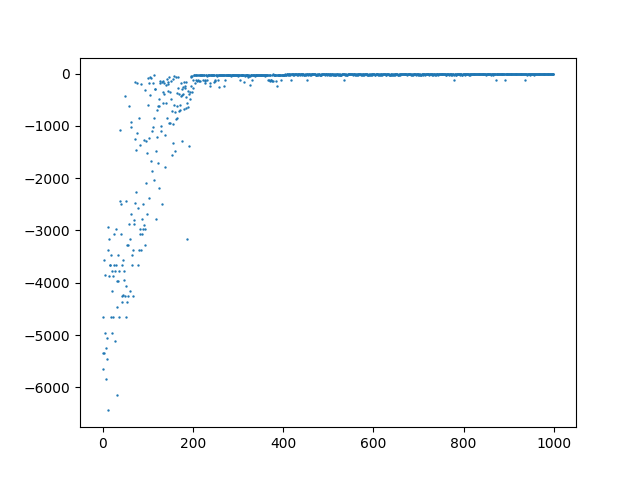
\includegraphics[width=0.4\textwidth]{Figure_1.png}}
	  \caption{}
	  \label{fig:oscil}
	\end{figure}
	
\begin{figure}[H]
	  \centering
	  \subfloat[Episode Reward of Q-learning ]{\label{fig:Per6A}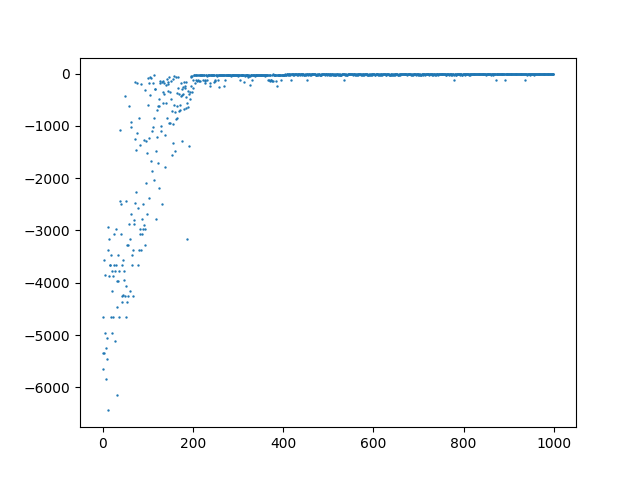
\includegraphics[width=0.4\textwidth]{Figure_1.png}}
	  \caption{}
	  \label{fig:oscil}
	\end{figure}
\subsection{Basic algorithm}
I implemented both agents with there Q-value fields represented by numpy marices. The state transfer equations of Sarsa and Q-learning are as follows respetively:

\begin{center}
    \begin{equation}
        Q(s,a) \xleftarrow[]{} (1-\alpha) Q(s,a) +\alpha (r+\gamma Q(s',a'_{\epsilon-greedy})
    \end{equation}
\end{center}

\begin{center}
    \begin{equation}
       Q(s,a) \xleftarrow[]{} (1-\alpha) Q(s,a) +\alpha (r+\gamma max_{a'}Q(s',a'_{\epsilon-greedy})
    \end{equation}
\end{center}

\subsection{Epsilon Decay Scheme}
\vspace{3mm}
Then I implemented an \begin{equation}
    \epsilon
\end{equation}-decay strategy as follow, so that it converges quite fast.

\begin{center}
    \begin{equation}
       \epsilon =\left  \begin{cases}
         1-0.0015 \times episode & episode < 200\quad \\
         0.5-0.005 \times episode & 200 \leq episode < 400 \quad \\
         0.1 - 0.0001 \times episode & otherwise \right
    \end{cases}
    \end{equation}
\end{center}

\begin{figure}[H]
	  \centering
	  \subfloat[epsilon-decay function]{\label{fig:Per6A}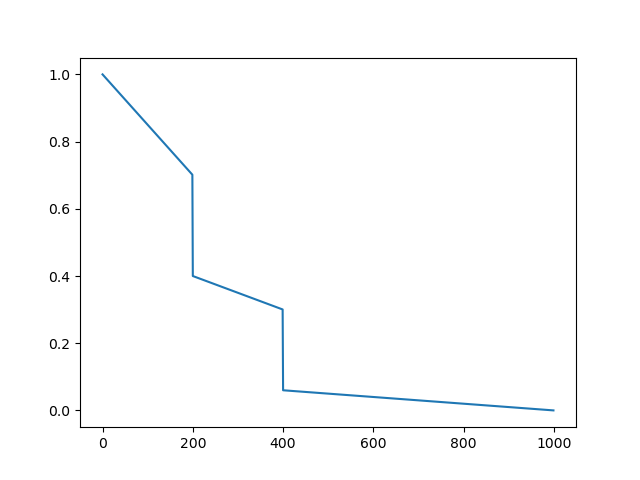
\includegraphics[width=0.4\textwidth]{decay.png}}
	  \caption{}
	  \label{fig:oscil}
	\end{figure}

\subsection{Results and Analysis}
As shown in the videos, sarsa and q-learning converges at different routes. Sarsa agent chooses to get as far away to the cliff as possible and walks along the edge of the map, while Q-learning agent chooses to walk the shortest path, which is really close to the cliff.
There are reasons for the differences:
For Q-learning, it updates Q(s, a) with the max value of Q(s
′
, ai). Although some directions’ Q value of
a grid may be low, maxai
(Q(s
′
, ai)) can still be large. In our example, although the Q value for each grid
on this path is small in the downward direction, the agent is still likely to choose move right due to the
seductive reward for moving directly to the target point.
For SARSA, this is because grid (1, 1) has a smaller Q value on the downward direction, which will
gradually reduce the Q value of the grid (0, 1) in its right direction. And when the agent arrive (0, 1), it’s
more likely to choose to move upward.

\subsection{Code}
\vspace{5mm}
	\lstinputlisting{agent.py}
	\vspace{3mm}
%%%%%%%%%%%%%%%%%%%%%%%%%%%%%%

%%%%%%%%%%%%%%%%%%%%%%%%%%%%%%


%%%%%%%%%%%%%%%%%%%%%%%%%%%%%%
%%%%%%%%%%%%%%%%%%%%%%%%%%%%%%
\newpage
\section{Task 2: Deep Reinforcement Learning}


\subsection{Preparation: Install Cuda to accelerate}
First, I installed cuda to the virtual environment, so that the training is process accelerated and I can train the model for more timesteps, which can be costly.
\vspace{3mm} 
\subsection{Hyper-parameters Tuning}

Then I tuned the  hyper-parameters as follows: learning rate = 3e-3, gamma = 0.99, start-e = 1, end-e = 0.01, to make the dqn converge. By training for 1000000 steps, I can see that it converges at about 1000 episodes, but the original number of steps,300000, is just not enough to go through so much episodes. Thanks to cuda, it seems not too costly to train so many steps, although it can certainly been improved to converge faster. A decay strategy similar to that implemented in Task1 can be helpful.

\begin{figure}[H]
	  \centering
	  \subfloat[Episodic Reward of 300000 timesteps ]{\label{fig:Per6A}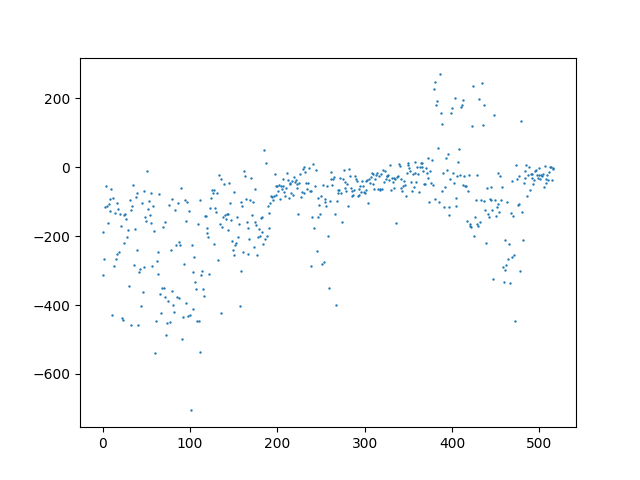
\includegraphics[width=0.4\textwidth]{Figure_3.png}}\\
	  \subfloat[Episodic Reward of 1000000 timesteps 3]{\label{fig:Per6A}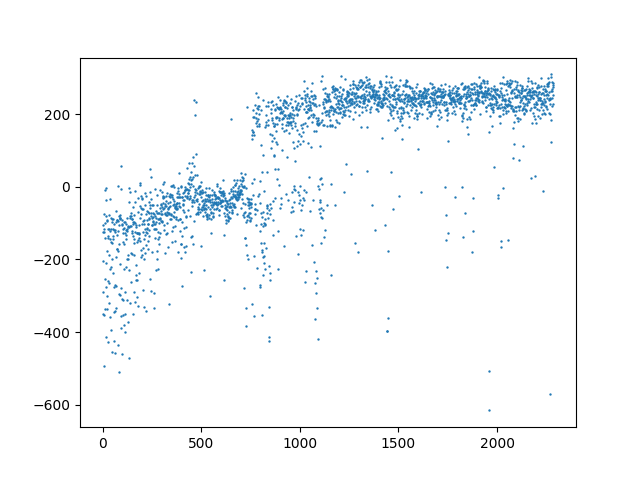
\includegraphics[width=0.4\textwidth]{Figure_5.png}}
	  \caption{}
	  \label{fig:oscil}
	\end{figure}

\subsection{Code}
\vspace{5mm}
	\lstinputlisting{dqn.py}
	\vspace{3mm}


%%%%%%%%%%%%%%%%%%%%%%%%%%%%%%
%%%%%%%%%%%%%%%%%%%%%%%%%%%%%%




\end{document} % DONE WITH DOCUMENT!


%%%%%%%%%%


% MATHMATICAL ENVIRONMENT
$ 8 = 2 \times 4 $

% CENTERED FORMULA
\[  \]

% NUMBERED EQUATION
\begin{equation}
	
\end{equation}

% ARRAY OF EQUATIONS (The splat supresses the numbering)
\begin{align*}
	
\end{align*}

% NUMBERED ARRAY OF EQUATIONS
\begin{align}
	
\end{align}

% ACCENTS
\dot{x} % dot
\ddot{x} % double dot
\bar{x} % bar
\tilde{x} % tilde
\vec{x} % vector
\hat{x} % hat
\acute{x} % acute
\grave{x} % grave
\breve{x} % breve
\check{x} % dot (cowboy hat)

% FONTS
\mathrm{text} % roman
\mathsf{text} % sans serif
\mathtt{text} % Typewriter
\mathbb{text} % Blackboard bold
\mathcal{text} % Caligraphy
\mathfrak{text} % Fraktur

\textbf{text} % bold
\textit{text} % italic
\textsl{text} % slanted
\textsc{text} % small caps
\texttt{text} % typewriter
\underline{text} % underline
\emph{text} % emphasized

\begin{tiny}text\end{tiny} % Tiny
\begin{scriptsize}text\end{scriptsize} % Script Size
\begin{footnotesize}text\end{footnotesize} % Footnote Size
\begin{small}text\end{small} % Small
\begin{normalsize}text\end{normalsize} % Normal Size
\begin{large}text\end{large} % Large
\begin{Large}text\end{Large} % Larger
\begin{LARGE}text\end{LARGE} % Very Large
\begin{huge}text\end{huge}   % Huge
\begin{Huge}text\end{Huge}   % Very Huge


% GENERATE TABLE OF CONTENTS AND/OR TABLE OF FIGURES
% These seem to have some issues with the "revtex4" document class.  To use, change
% the very first line of this document to "article" like this:
% \documentclass[aps,letterpaper,10pt]{article}
\tableofcontents
\listoffigures
\listoftables

% INCLUDE A HYPERLINK OR URL
\url{http://www.derekhildreth.com}
\href{http://www.derekhildreth.com}{Derek Hildreth's Website}

% FOR MORE, REFER TO THE "LINUX CHEAT SHEET.PDF" FILE INCLUDED!
